\documentclass[a4paper,12pt]{article} % This defines the style of your paper

\usepackage[top = 2.5cm, bottom = 2.5cm, left = 2.5cm, right = 2.5cm]{geometry} 

% Unfortunately, LaTeX has a hard time interpreting German Umlaute. The following two lines and packages should help. If it doesn't work for you please let me know.
\usepackage[T1]{fontenc}
\usepackage[utf8]{inputenc}
\usepackage{subcaption}

% The following two packages - multirow and booktabs - are needed to create nice looking tables.
\usepackage{multirow} % Multirow is for tables with multiple rows within one cell.
\usepackage{booktabs} % For even nicer tables.
\usepackage{amsmath}

% As we usually want to include some plots (.pdf files) we need a package for that.
\usepackage{graphicx} 
\usepackage{rotating}



% The default setting of LaTeX is to indent new paragraphs. This is useful for articles. But not really nice for homework problem sets. The following command sets the indent to 0.
\usepackage{setspace}
\setlength{\parindent}{0in}

% Package to place figures where you want them.
\usepackage{float}

% The fancyhdr package let's us create nice headers.
\usepackage{fancyhdr}

\usepackage[utf8]{inputenc}
\usepackage[portuguese]{babel}
\usepackage{makecell}
\usepackage{listings}
\usepackage{xcolor}

\definecolor{codegreen}{rgb}{0,0.6,0}
\definecolor{codegray}{rgb}{0.5,0.5,0.5}
\definecolor{codepurple}{rgb}{0.58,0,0.82}
\definecolor{backcolour}{rgb}{0.95,0.95,0.92}

\lstdefinestyle{mystyle}{
    backgroundcolor=\color{backcolour},   
    commentstyle=\color{codegreen},
    keywordstyle=\color{magenta},
    numberstyle=\tiny\color{codegray},
    stringstyle=\color{codepurple},
    basicstyle=\ttfamily\footnotesize,
    breakatwhitespace=false,         
    breaklines=true,                 
    captionpos=b,                    
    keepspaces=true,                 
    numbers=left,                    
    numbersep=5pt,                  
    showspaces=false,                
    showstringspaces=false,
    showtabs=false,                  
    tabsize=2
}
\lstset{style=mystyle}
\renewcommand{\arraystretch}{1.5}

\pagestyle{fancy} % With this command we can customize the header style.

\fancyhf{} % This makes sure we do not have other information in our header or footer.

\lhead{\footnotesize Homework 2}% \lhead puts text in the top left corner. \footnotesize sets our font to a smaller size.

%\rhead works just like \lhead (you can also use \chead)
\rhead{\footnotesize Joana Pimenta, Rodrigo Laia} %<---- Fill in your lastnames.

% Similar commands work for the footer (\lfoot, \cfoot and \rfoot).
% We want to put our page number in the center.
\cfoot{\footnotesize \thepage} 

\begin{document}

\thispagestyle{empty} % This command disables the header on the first page. 

\begin{tabular}{p{15.5cm}} % This is a simple tabular environment to align your text nicely 
{\large \bf Aprendizagem} \\
Instituto Superior Técnico \\ setembro de 2023  \\ \\ 
\hline % \hline produces horizontal lines.
\\
\end{tabular} % Our tabular environment ends here.

\vspace*{0.3cm} % Now we want to add some vertical space in between the line and our title.

\begin{center} % Everything within the center environment is centered.
	{\Large \bf Homework 2 - Report} % <---- Don't forget to put in the right number
	\vspace{2mm}
	
        % YOUR NAMES GO HERE
	{\bf Joana Pimenta (103730), Rodrigo Laia (102674) } % <---- Fill in your names here!
		
\end{center}  

\vspace{0.4cm}

%%%%%%%%%%%%%%%%%%%%%%%%%%%%%%%%%%%%%%%%%%%%%%%%
%%%%%%%%%%%%%%%%%%%%%%%%%%%%%%%%%%%%%%%%%%%%%%%%

% Up until this point you only have to make minor changes for every week (Number of the homework). Your write up essentially starts here.

\section*{Pen and Paper}
\begin{enumerate}

\item 
\begin{enumerate}
\item
${y_1,y_2} , {y_3,y_4}$ and $y_5$ independent $\implies p(y_1,y_2,y_3,y_4,y_5) = p(y_1,y_2)\times p(y_3,y_4)\times p(y_5)$ \\

Fórmulas utilizadas:
\begin{equation}
    P(y_6=H|\vec{x}) = \frac{P(\vec{x}|y_6=H)}{P(\vec{x})}
\end{equation}

\begin{equation}
    P(\vec{x}|\mu, \sigma^2) = \frac{1}{(2\pi)^{m/2} \sqrt{|\Sigma|}}e^{-\frac{1}{2}(\vec{x}-\vec{\mu})^T \cdot \Sigma^{-1} \cdot (\vec{x}-\vec{\mu})}
\end{equation}

\begin{equation}
    \vec{\mu} = \begin{bmatrix} E(y_1) \\ E(y_2)  \end{bmatrix}
\end{equation}

\begin{equation}
    cov(x,y) = \sum_{i=1}^{n} \frac{(x_i - E(x))(y_i - E(y))}{n}
\end{equation}

\begin{equation}
    \Sigma = \begin{bmatrix} cov(y_1,y_2) & cov(y_1,y_1) \\ cov(y_2,y_1) & cov(y_2,y_2) \end{bmatrix}
\end{equation}

\begin{equation}
    |\Sigma| = cov(y_1,y_2) \cdot cov(y_2,y_1) - cov(y_1,y_1) \cdot cov(y_2,y_2)
\end{equation}

\begin{equation}
    \Sigma^{-1} =  \frac{1}{|\Sigma|} \cdot \begin{bmatrix} cov(y_2,y_2) & -cov(y_1,y_2) \\ -cov(y_2,y_1) & cov(y_1,y_1) \end{bmatrix} 
\end{equation}

Parâmetros das gaussianas multivariadas: \\ \\
Classe A:
\begin{equation*} 
    \vec{\mu}_A = \begin{bmatrix} 0.24 \\ 0.52 \end{bmatrix} 
\end{equation*}
\begin{equation*} 
    \Sigma_A = \begin{bmatrix} 0.004267 & -0.0064 \\ -0.0064 & 0.02240 \end{bmatrix}
\end{equation*}

\begin{equation*} 
    |\Sigma|_A = 5.4613 \cdot 10^{-5}
\end{equation*}

\begin{equation*} 
\Sigma^{-1}_A = \begin{bmatrix} 410.1563 & -117.1875 \\ -117.1875 & 78.125 \end{bmatrix}
\end{equation*}

\begin{equation*}
    P(\vec{x}|A) = N(\vec{x}|\mu_{A},\Sigma_{A}) = \frac{1}{(2\pi)^{m/2} \sqrt{|\Sigma_{A}|}}e^{-\frac{1}{2}(\vec{x}-\vec{\mu}_A)^T \cdot \Sigma_A^{-1} \cdot (\vec{x}-\vec{\mu}_A)}
\end{equation*}

Classe B: \\ \\ 
\begin{equation*}
    \vec{\mu}_B = \begin{bmatrix} 0.5925 \\ 0.3275 \end{bmatrix}  
\end{equation*}
\begin{equation*}
    \Sigma_B = \begin{bmatrix} 0.01717 & -0.00732 \\ -0.00732 & 0.02362 \end{bmatrix} 
\end{equation*} \\
\begin{equation*}
    |\Sigma|_B = 3.519 \cdot 10^{-4} 
\end{equation*}
\begin{equation*}
    \Sigma^{-1}_B = \begin{bmatrix} 67.1101 & 20.7954 \\ 20.7954 & 48.7831 \end{bmatrix}
\end{equation*}
\begin{equation*}
    P(\vec{x}|B) = N(\vec{x}|\mu_{B},\Sigma_{B}) = \frac{1}{(2\pi)^{m/2} \sqrt{|\Sigma_{B}|}}e^{-\frac{1}{2}(\vec{x}-\vec{\mu}_B)^T \cdot \Sigma_B^{-1} \cdot (\vec{x}-\vec{\mu}_B)}
\end{equation*}


\textbf{Probabilidades para $\{y_3,y_4\}$ condicionadas a A e B :}
\\ \\
Classe A:
\begin{table}[H]
\centering
\begin{tabular}{c|c|c|} 
    \cline{2-3}
                                 & $y_3=0$ & $y_3=1$ \\ \hline
    \multicolumn{1}{|c|}{$y_4=0$} & P=0    & P=1/3  \\ \hline
    \multicolumn{1}{|c|}{$y_4=1$} & P=1/3  & P=1/3  \\ \hline
    \end{tabular}
    \caption{Probabilidades para ${y_3,y_4}$ condicionadas a A}
\end{table}

Classe B:

\begin{table}[H]
    \centering
    \begin{tabular}{c|c|c|} 
        \cline{2-3}
                                     & $y_3=0$ & $y_3=1$ \\ \hline
        \multicolumn{1}{|c|}{$y_4=0$} & P=1/2    & P=1/4  \\ \hline
        \multicolumn{1}{|c|}{$y_4=1$} & P=1/4  & P=0  \\ \hline
        \end{tabular}
        \caption{Probabilidades para ${y_3,y_4}$ condicionadas a B}
    \end{table}

\textbf{Probabilidades para $\{y_5\}$ condicionadas a A e B :}
\\ \\
Classe A:

\begin{equation*}
    P(y_5=0|A) = 1/3
\end{equation*}

\begin{equation*}
    P(y_5=1|A) = 1/3
\end{equation*}

\begin{equation*}
    P(y_5=2|A) = 1/3
\end{equation*}

Classe B:

\begin{equation*}
    P(y_5=0|A) = 1/4
\end{equation*}

\begin{equation*}
    P(y_5=1|A) = 1/2
\end{equation*}

\begin{equation*}
    P(y_5=2|A) = 1/4
\end{equation*}

Priors:
\begin{equation*}    
    P(A) = \frac{3}{7}
\end{equation*}

\begin{equation*}    
    P(B) = \frac{4}{7}
\end{equation*}



\item Uma vez que o denominador é o mesmo para todas para saber qual a classe mais provável, basta comparar os numeradores das probabilidades.

\begin{equation*}
    \begin{aligned}
        P(A|\vec{x}_8) & = \frac{P(\vec{x}_8|A) \cdot P(A)}{P(\vec{x}_8)} \\
                       & = \frac{P(y_1=0.38,y_2=0.52|A) \cdot P(y_3=0,y_4=1|A) \cdot P(y_5=0|A) \cdot P(A)}{P(\vec{x}_8)} \\
                       & = \frac{\frac{3}{7} \cdot 0.3868 \cdot \frac{1}{3} \cdot \frac{1}{3}}{P(\vec{x}_8)} \\
                       & = \frac{0.018}{P(\vec{x}_8)}
    \end{aligned}
\end{equation*}
    
\begin{equation*}
    \begin{aligned}
        P(B|\vec{x}_8) & = \frac{P(\vec{x}_8|B) \cdot P(B)}{P(\vec{x}_8)} \\
                       & = \frac{P(y_1=0.38,y_2=0.52|B) \cdot P(y_3=0,y_4=1|B) \cdot P(y_5=0|B) \cdot P(B)}{P(\vec{x}_8)} \\
                       & = \frac{\frac{4}{7} \cdot 1.7678 \cdot \frac{1}{4} \cdot \frac{1}{4}}{P(\vec{x}_8)} \\
                       & = \frac{0.063}{P(\vec{x}_8)}
    \end{aligned}
\end{equation*}

Como $P(A|\vec{x}_8) < P(B|\vec{x}_8)$, então $\vec{x}_8$ é classificado como B.

\begin{equation*}
    \begin{aligned}
        P(A|\vec{x}_9) & = \frac{P(\vec{x}_9|A) \cdot P(A)}{P(\vec{x}_9)} \\
                       & = \frac{P(y_1=0.42,y_2=0.59|A) \cdot P(y_3=0,y_4=1|A) \cdot P(y_5=0|A) \cdot P(A)}{P(\vec{x}_9)} \\
                       & = \frac{\frac{3}{7} \cdot 0.1013 \cdot \frac{1}{3} \cdot \frac{1}{3}}{P(\vec{x}_9)} \\
                       & = \frac{0.0048}{P(\vec{x}_9)}
    \end{aligned}
\end{equation*}
    
\begin{equation*}
    \begin{aligned}
        P(B|\vec{x}_8) & = \frac{P(\vec{x}_8|B) \cdot P(B)}{P(\vec{x}_8)} \\
                       & = \frac{P(y_1=0.42,y_2=0.59|B) \cdot P(y_3=0,y_4=1|B) \cdot P(y_5=1|B) \cdot P(B)}{P(\vec{x}_8)} \\
                       & = \frac{\frac{4}{7} \cdot 1.4927 \cdot \frac{1}{4} \cdot \frac{1}{2}}{P(\vec{x}_8)} \\
                       & = \frac{0.1066}{P(\vec{x}_8)}
    \end{aligned}
\end{equation*}

Como $P(A|\vec{x}_9) < P(B|\vec{x}_9)$, então $\vec{x}_9$ é classificado como B. 

\item 
Assumindo o critério de Maximum Likelihood, para classificar uma observação apenas interessam as probabilidades $P(\vec{x}|A)$ e $P(\vec{x}|B)$:
\begin{equation*}
    h = argmax(P(\vec{x}_8|h))
\end{equation*}

Considerando diferentes thresholds $\theta$ para as probabilidades é possível maximizar a accuracy do nosso classificador:

\begin{equation*}
    f(\vec{x}_8) = \begin{cases} 
        A & \text{se } P(A|\vec{x}_8) > \theta \\
        B &  \text{otherwise}
     \end{cases}
\end{equation*}


\begin{equation*}
    P(\vec{x}_8|A) = P(y_1=0.38,y_2=0.52|A) \cdot P(y_3=0,y_4=1|A) \cdot P(y_5=0|A) = 0.043
\end{equation*}

\begin{equation*}
    P(\vec{x}_9|A) = P(y_1=0.42,y_2=0.59|A) \cdot P(y_3=0,y_4=1|A) \cdot P(y_5=0|A) = 0.0113
\end{equation*}

Assumindo o critério de maximum Likelihood os priors são todos iguais.
Escolhendo qualquer valor no intervalo (0.0113,0.043) como threshold $\theta$, a accuracy do classificador é de 100\% para estas observações de teste.

\end{enumerate}

\item

As  fórmulas utilizadas neste exercício são:

\begin{equation*}
    \hat{z} = \frac{\sum_{i=1}^{k} w_i \cdot z_{i}}{\sum_{i=1}^{k} w_i}
\end{equation*}

\begin{equation*}
    MAE = \frac{\frac{1}{n}}{\sum_{i=1}^{n} |z_i - \hat{z}|}
\end{equation*}

Para discretizar a variável $y_2$, considerando equal-width, é necessário dividir o intervalo $[0,1]$ em 2 partes iguais. 
Assim, os intervalos são: $[0,0.5]$, $[0.5,1]$. \\

Para cada observação, $y_2$ pode assumir os valores 0 ou 1, consoante o intervalo em que se encontra o seu valor. \\

\begin{table}[H]
    \centering
    \begin{tabular}{c|ccccccccc}
    $y_2$     & 0.36 & 0.48 & 0.72 & 0.11 & 0.39 & 0.28 & 0.53 & 0.52 & 0.59 \\ \hline
    $y_{2 new}$ & 0    & 0    & 1    & 0    & 0    & 0    & 1    & 1    & 1   
    \end{tabular}
\end{table}

(a)
Em 3-Fold cross-validation o dataset é dividido em 3 partes iguais. Duas delas são usadas para teste e uma para treino.

Porque não há shuffling:

\begin{table}[H]
    \begin{minipage}[b]{0.3\linewidth}
    \centering
    \captionof{table}{1º Fold}
    \begin{tabular}{cccccc}
        $x_1$ & 0 & 1 & 1 & 0 & A \\ \hline
        $x_2$ & 0 & 1 & 0 & 1 & A \\ \hline
        $x_3$ & 1 & 0 & 1 & 2 & A
        \end{tabular}
    \end{minipage}
    \hfill
    \begin{minipage}[b]{0.3\linewidth}
    \centering
    \captionof{table}{2º Fold}
    \begin{tabular}{cccccc}
        $x_1$ & 0 & 0 & 0 & 1 & B \\ \hline
        $x_2$ & 0 & 0 & 0 & 0 & B \\ \hline
        $x_3$ & 0 & 1 & 0 & 2 & B
        \end{tabular}
    \end{minipage}
    \hfill
    \begin{minipage}[b]{0.3\linewidth}
    \centering
    \captionof{table}{3º Fold}
    \begin{tabular}{cccccc}
        $x_1$ & 1 & 0 & 1 & 1 & B \\ \hline
        $x_2$ & 1 & 0 & 1 & 0 & A \\ \hline
        $x_3$ & 1 & 0 & 1 & 1 & B
        \end{tabular}
    \end{minipage}
    \hfill

\end{table}

(b)

\begin{table}[H]
    \centering
    \begin{tabular}{cccccccc}
    D  & $y_1$   & $y_2$ & $y_3$ & $y_4$ & $y_5$ & $y_6$ &         \\ \hline
    $x_1$ & 0.24 & 0  & 1  & 1  & 0  & A  & \multirow{6}{*}{TRAIN} \\
    $x_2$ & 0.16 & 0  & 1  & 0  & 1  & A  &                        \\
    $x_3$ & 0.32 & 1  & 0  & 1  & 2  & A  &                        \\
    $x_4$ & 0.54 & 0  & 0  & 0  & 1  & B  &                        \\
    $x_5$ & 0.66 & 0  & 0  & 0  & 0  & B  &                        \\
    $x_6$ & 0.76 & 0  & 1  & 0  & 2  & B  &                        \\ \hline
    $x_7$ & 0.41 & 1  & 0  & 1  & 1  & B  & \multirow{3}{*}{TEST}  \\
    $x_8$ & 0.38 & 1  & 0  & 1  & 0  & A  &                        \\
    $x_9$ & 0.42 & 1  & 0  & 1  & 1  & B  &                       
    \end{tabular}
\end{table}

Para $x_7$:

\begin{table}[H]
    \centering
    \begin{tabular}{c|cccccc}
    d      & $x_1$ & $x_2$ & $x_3$ & $x_4$ & $x_5$ & $x_6$ \\ \hline
    $x_7$  & 4     & 4     & 2     & 2     & 3     & 4    
    \end{tabular}
\end{table}

As observações com menor distância de Hamming são $x_3$, $x_4$ e $x_5$. O output previsto pelo kNN é dado por 

\begin{equation*}
    \hat{z}_{7} = \frac{1/2 \cdot 0.32 + 1/2 \cdot 0.54 + 1/3 \cdot 0.66}{1/2 + 1/2 + 1/3} = 0.4875
\end{equation*}

Para $x_8$:

\begin{table}[H]
    \centering
    \begin{tabular}{c|cccccc}
    d      & $x_1$ & $x_2$ & $x_3$ & $x_4$ & $x_5$ & $x_6$ \\ \hline
    $x_8$  & 2     & 4     & 1     & 4     & 3     & 5    
    \end{tabular}
    \end{table}

As observações com menor distância de Hamming são $x_1$, $x_3$ e $x_5$. O output previsto pelo kNN é dado por 

\begin{equation*}
    \hat{z}_{8} = \frac{1/2 \cdot 0.24 + 1 \cdot 0.32 + 1/3 \cdot 0.66}{1/2 + 1 + 1/3} = 0.36
\end{equation*}

Como as observações $x_7$ e $x_9$ são iguais, o output previsto pelo kNN para  $x_9$ é igual ao output previsto para $x_7$.

\begin{equation*}
    \hat{z}_{9} = \hat{z}_{7} = 0.4875
\end{equation*}

Por fim, o MAE deste classificador é dado por:

\begin{equation*}
    MAE = \frac{1}{3} \cdot (|0.41 - 0.4875| + |0.38 - 0.36| + |0.42 - 0.4875|) = 0.055
\end{equation*}

\end{enumerate}

\clearpage
\section*{Programming - Código Python e Resultados Obtidos}

\begin{enumerate}
    \item O objetivo deste exercício é comparar a performance de dois classificadores
    (Naive Bayes com distribuição Gaussiana e kNN) para o dataset.
    
        (a) Boxplots para as accuracies obtidas para GaussianNB e kNN:
        \begin{figure}[H]
            \centering
            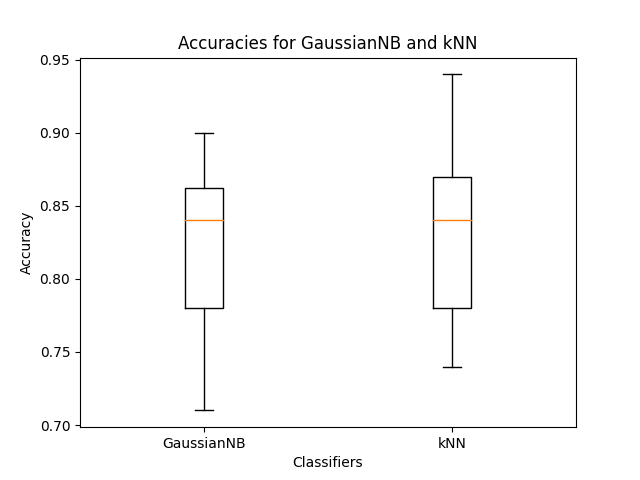
\includegraphics[width=0.8\textwidth]{ex1a_boxplot.png}
            \caption{Boxplot para as accuracies obtidas para GaussianNB e kNN}
            \label{fig:boxplot}
        \end{figure}
        Conclui-se que apesar do o classificador kNN atingir accuracies maiores do que 
        o GaussianNB, a mediana de ambos é quase igual. Além disso, o kNN tem accuracies ligeiramente mais dispersas 
        (a sua distância interquartis é maior). A amplitude do boxplot é parecida para ambos os classificadores. 
        \\ \\
        Código utilizado:
        \begin{lstlisting}[language=Python]
### Exercise 1 ###

#a)

acc_folds_gauss = []
acc_folds_knn = []
folds = StratifiedKFold(n_splits=10, shuffle=True, random_state=0)

# Gaussian Naive Bayes
gaussNB = GaussianNB()

# KNN
knn_predictor = KNeighborsClassifier(n_neighbors=5)

# iterate per fold
for train_k, test_k in folds.split(features, target):
    X_train, X_test = features.iloc[train_k], features.iloc[test_k]
    y_train, y_test = target.iloc[train_k], target.iloc[test_k]
    
    ## train and assess
    gaussNB.fit(X_train, y_train)
    y_pred_gauss = gaussNB.predict(X_test)
    acc_folds_gauss.append(round(metrics.accuracy_score(y_test, y_pred_gauss),2))
    
    knn_predictor.fit(X_train, y_train)
    y_pred_knn = knn_predictor.predict(X_test)
    acc_folds_knn.append(round(metrics.accuracy_score(y_test, y_pred_knn),2))

print("Fold accuracies GaussianNB:", acc_folds_gauss)
print("Fold accuracies kNN:", acc_folds_knn)

plt.boxplot([acc_folds_gauss, acc_folds_knn], labels=['GaussianNB', 'kNN'])
plt.title('Accuracies for GaussianNB and kNN')
plt.xlabel('Classifiers')
plt.ylabel('Accuracy')
plt.savefig('ex1a_boxplot.png')
plt.show()
        \end{lstlisting}

    
    (b) Concluímos que a hipótese nula (H0: kNN não é estatisticamente superior a GaussianNB) não é rejeitada, uma vez que o p-value é maior do que 0.05, logo kNN não é estatisticamente superior a GaussianNB.
    \\ \\
    Código utilizado:
    \begin{lstlisting}[language=Python]
#b) 
Null Hypothesis: kNN is not statistically superior to GaussianNB
hypothesis = stats.ttest_rel(acc_folds_knn, acc_folds_gauss, alternative='greater')

if hypothesis[1] < 0.05:
    print("The null hypothesis is rejected and kNN is statistically superior to GaussianNB")
    
else:
    print("The null hypothesis is not rejected and there is no statistical superiority between kNN and GaussianNB")
    \end{lstlisting}

    \item O objetivo deste exercício é comparar a performance de dois classificadores : kNN com k=1 e kNN com k=5. 
    Assim, calculamos as matrizes de confusão para os dados de cada uma das 10 iterações, somámos os valores de cada célula obtendo duas matrizes de confusão cumulativas que subtraímos uma a outra (kNN com k=1 - kNN com k=5).
    \begin{figure}[H]
        \centering
        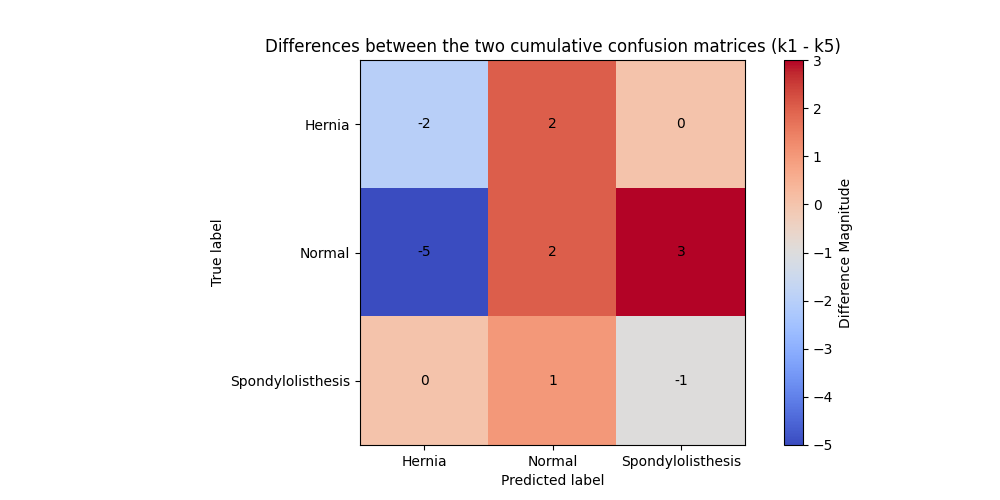
\includegraphics[width=0.8\textwidth]{ex2_cummatrix.png}
        \caption{Matriz de confusão cumulativa para kNN com k=1 - kNN com k=5}
        \label{fig:ex2a}
    \end{figure}

    CONCLUSÕESSSSS FAAAAAFIIIIIII

    \begin{lstlisting}[language=Python]
        ############ Exercise 2 ############

        #Initialize the cumulative confusion matrices
        cum_conf_matrix1 = np.zeros((3,3))
        cum_conf_matrix5 = np.zeros((3,3))
        
        for train_k, test_k in folds.split(features, target):
            X_train, X_test = features.iloc[train_k], features.iloc[test_k]
            y_train, y_test = target.iloc[train_k], target.iloc[test_k]
            
            ## train and assess
            knn1 = KNeighborsClassifier(n_neighbors=1,weights='uniform',metric='euclidean')
            knn5 = KNeighborsClassifier(n_neighbors=5,weights='uniform',metric='euclidean')
        
            knn1.fit(X_train, y_train)
            knn5.fit(X_train, y_train)
        
            # Make predictions
            y_pred1 = knn1.predict(X_test)
            y_pred5 = knn5.predict(X_test)
        
            # Calculate confusion matrices
            conf_matrix1 = confusion_matrix(y_test, y_pred1)
            conf_matrix5 = confusion_matrix(y_test, y_pred5)
        
            # Calculate cumulative confusion matrices
            cum_conf_matrix1 += conf_matrix1
            cum_conf_matrix5 += conf_matrix5
        
        #Calculate the difference between the two confusion matrices
        conf_matrix_diff = cum_conf_matrix1 - cum_conf_matrix5
        
        confusion1 = pd.DataFrame(conf_matrix_diff, index=knn1.classes_, columns=['Predicted Hernia', 'Predicted Normal', 'Predicted Spondylolisthesis'])
        
        #Plotting 
        plt.figure(figsize=(10, 5))
        heatmap = plt.imshow(conf_matrix_diff,cmap="coolwarm", interpolation='nearest')
        plt.title('Differences between the two cumulative confusion matrices (k1 - k5)')
        plt.xlabel('Predicted label')
        plt.xticks([0, 1, 2], ['Hernia', 'Normal', 'Spondylolisthesis'])
        plt.yticks([0, 1, 2], ['Hernia', 'Normal', 'Spondylolisthesis'])
        plt.ylabel('True label')
        
        cbar = plt.colorbar(heatmap)
        cbar.set_label('Difference Magnitude', rotation=90)
        
        for i in range(conf_matrix_diff.shape[0]):
            for j in range(conf_matrix_diff.shape[1]):
                plt.text(j, i, str(int(conf_matrix_diff[i, j])), ha='center', va='center', color='black')
        plt.savefig('ex2_cummatrix.png')
        plt.show()
    \end{lstlisting}
    
\item Apesar de ser uma abordagem fácil e rápida, o Naive Bayes apresenta algumas desvantagens para este dataset. 
Um problema é, por exemplo, a suposição de que as features têm uma distribuição Gaussiana. Para podermos visualizar a distribuição
experimental destes features fizemos um histograma para cada um deles e concluímos que a maioria não tem uma distribuição Gaussiana, especialmente por exemplo a feature $degree\_Spondylolisthesis$.

\begin{figure}[H]
    \centering
    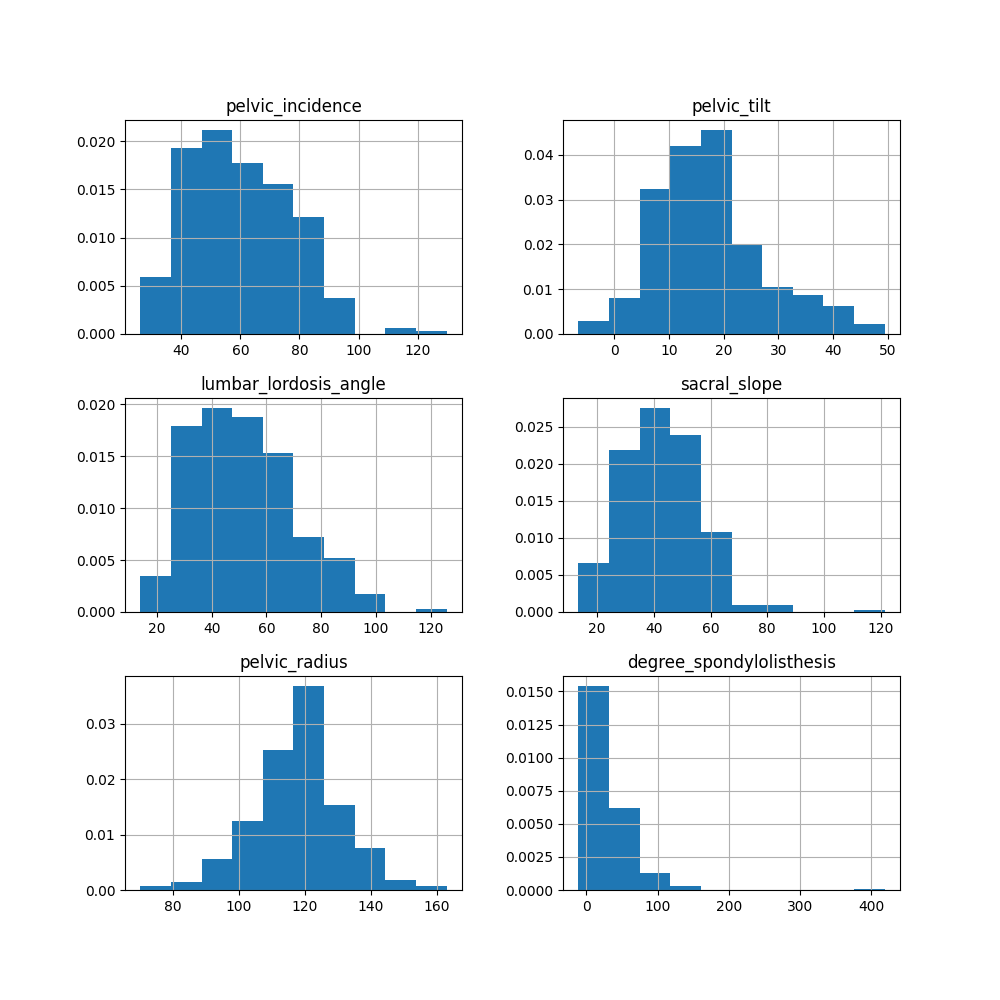
\includegraphics[width=0.8\textwidth]{ex3_1_hist.png}
    \caption{Histogramas para cada feature}
    \label{fig:ex3_histograms}
\end{figure}


Código utilizado:

\begin{lstlisting}[language=Python]
    ############ Exercise 3 ############
    #1. The dataset is not normally distributed, which is an assumption of the Naive Bayes classifier.
    #Histograms for each feature:
    features.hist(figsize=(10,10),density=True)
    plt.savefig('ex3_1_hist.png')
    plt.show()
\end{lstlisting}

Para além disso, outro exemplo de uma dificuldade do Naive Bayes é a suposição de que as features são independentes. Para avaliar 
se estas featuras eram independentes ou não, fizemos a seguinte matriz de correlação:

\begin{figure}[H]
    \centering
    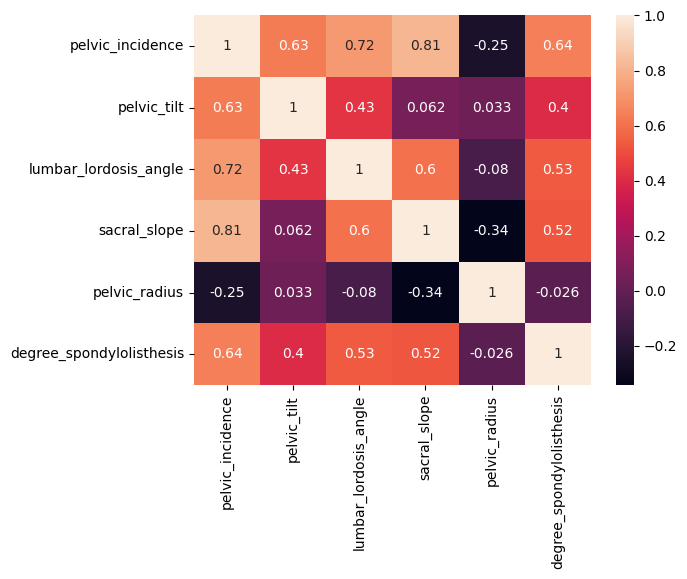
\includegraphics[width=0.8\textwidth]{ex3_3_coormatrix.png}
    \caption{Matriz de correlação}
    \label{fig:ex3_corr}
\end{figure}

Ao observar a matriz de correlação, concluímos que apesar de algumas features se encontrarem muito pouco
correladas, podendo por isso ser aproximadas como independentes (como por exemplo $pelvic\_radius$ e $pelvic\_tilt$), há outras
que se encontram bastante correladas e consequentemente não podem ser aproximadas como independentes (como por exemplo $pelvic\_incidence$ e $sacral\_slope$).

Código utilizado:


\end{enumerate}

\end{document}
